\documentclass[14pt]{extbook}
\usepackage{multicol, enumerate, enumitem, hyperref, color, soul, setspace, parskip, fancyhdr} %General Packages
\usepackage{amssymb, amsthm, amsmath, bbm, latexsym, units, mathtools} %Math Packages
\everymath{\displaystyle} %All math in Display Style
% Packages with additional options
\usepackage[headsep=0.5cm,headheight=12pt, left=1 in,right= 1 in,top= 1 in,bottom= 1 in]{geometry}
\usepackage[usenames,dvipsnames]{xcolor}
\usepackage{dashrule}  % Package to use the command below to create lines between items
\newcommand{\litem}[1]{\item#1\hspace*{-1cm}\rule{\textwidth}{0.4pt}}
\pagestyle{fancy}
\lhead{Progress Quiz 8}
\chead{}
\rhead{Version A}
\lfoot{4553-3922}
\cfoot{}
\rfoot{Fall 2020}
\begin{document}

\begin{enumerate}
\litem{
Determine the horizontal and/or oblique asymptotes in the rational function below.\[ f(x) = \frac{12x^{3} -1 x^{2} -80 x -75}{3x^{2} -7 x -20} \]\begin{enumerate}[label=\Alph*.]
\item \( \text{Oblique Asymptote of } y = 4x + 9. \)
\item \( \text{Horizontal Asymptote of } y = 4.000 \text{ and Oblique Asymptote of } y = 4x + 9 \)
\item \( \text{Horizontal Asymptote of } y = 0 \)
\item \( \text{Horizontal Asymptote of } y = 4.000  \)
\item \( \text{Horizontal Asymptote at } y = 4.000 \)

\end{enumerate} }
\litem{
Which of the following functions \textit{could} be the graph below?
\begin{center}
    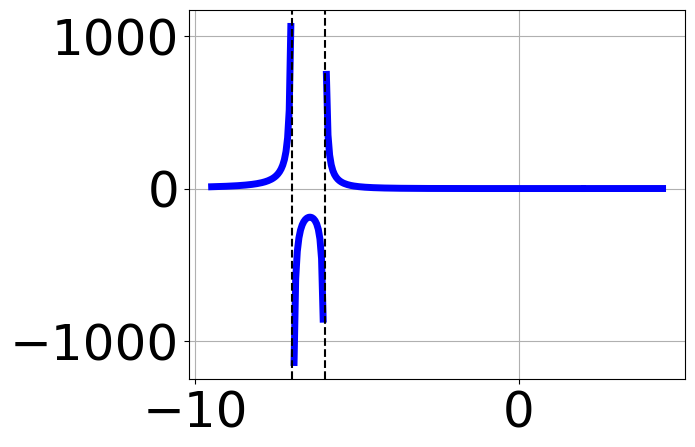
\includegraphics[width=0.5\textwidth]{../Figures/identifyGraphOfRationalFunctionCopyA.png}
\end{center}
\begin{enumerate}[label=\Alph*.]
\item \( f(x)=\frac{x^{3} -9 x^{2} +11 x + 21}{x^{3} -39 x -70} \)
\item \( f(x)=\frac{x^{3} -4 x^{2} -15 x + 18}{x^{3} -39 x + 70} \)
\item \( f(x)=\frac{x^{3} +9 x^{2} +11 x -21}{x^{3} -39 x + 70} \)
\item \( f(x)=\frac{x^{3} -9 x^{2} +11 x + 21}{x^{3} -39 x -70} \)
\item \( \text{None of the above are possible equations for the graph.} \)

\end{enumerate} }
\litem{
Determine the vertical asymptotes and holes in the rational function below.\[ f(x) = \frac{12x^{3} +79 x^{2} +144 x + 80}{9x^{2} -16} \]\begin{enumerate}[label=\Alph*.]
\item \( \text{Holes at } x = 1.333 \text{ and } x = -1.333 \text{ with no vertical asymptotes.} \)
\item \( \text{Vertical Asymptotes of } x = 1.333 \text{ and } x = -1.333 \text{ with no holes.} \)
\item \( \text{Vertical Asymptote of } x = 1.333 \text{ and hole at } x = -1.333 \)
\item \( \text{Vertical Asymptotes of } x = 1.333 \text{ and } x = -1.25 \text{ with a hole at } x = -1.333 \)
\item \( \text{Vertical Asymptote of } x = 1.333 \text{ and hole at } x = -1.333 \)

\end{enumerate} }
\litem{
Determine the vertical asymptotes and holes in the rational function below.\[ f(x) = \frac{12x^{3} -13 x^{2} -5 x + 6}{8x^{2} +6 x -9} \]\begin{enumerate}[label=\Alph*.]
\item \( \text{Vertical Asymptotes of } x = -1.5 \text{ and } x = 0.75 \text{ with no holes.} \)
\item \( \text{Vertical Asymptotes of } x = -1.5 \text{ and } x = -0.667 \text{ with a hole at } x = 0.75 \)
\item \( \text{Holes at } x = -1.5 \text{ and } x = 0.75 \text{ with no vertical asymptotes.} \)
\item \( \text{Vertical Asymptote of } x = 1.5 \text{ and hole at } x = 0.75 \)
\item \( \text{Vertical Asymptote of } x = -1.5 \text{ and hole at } x = 0.75 \)

\end{enumerate} }
\litem{
Determine the horizontal and/or oblique asymptotes in the rational function below.\[ f(x) = \frac{6x^{3} -13 x^{2} -21 x + 18}{3x^{2} +13 x -10} \]\begin{enumerate}[label=\Alph*.]
\item \( \text{Horizontal Asymptote of } y = 2.0  \)
\item \( \text{Horizontal Asymptote at } y = -5.0 \)
\item \( \text{Oblique Asymptote of } y = 2x -13. \)
\item \( \text{Horizontal Asymptote of } y = 2.0 \text{ and Oblique Asymptote of } y = 2x -13 \)
\item \( \text{Horizontal Asymptote of } y = -5.0 \text{ and Oblique Asymptote of } y = 2x -13 \)

\end{enumerate} }
\litem{
Determine the horizontal and/or oblique asymptotes in the rational function below.\[ f(x) = \frac{9x^{3} -12 x^{2} -11 x + 10}{3x^{2} +10 x -8} \]\begin{enumerate}[label=\Alph*.]
\item \( \text{Horizontal Asymptote at } y = -4.0 \)
\item \( \text{Horizontal Asymptote of } y = 3.0 \text{ and Oblique Asymptote of } y = 3x -14 \)
\item \( \text{Horizontal Asymptote of } y = 3.0  \)
\item \( \text{Oblique Asymptote of } y = 3x -14. \)
\item \( \text{Horizontal Asymptote of } y = -4.0 \text{ and Oblique Asymptote of } y = 3x -14 \)

\end{enumerate} }
\litem{
Which of the following functions \textit{could} be the graph below?
\begin{center}
    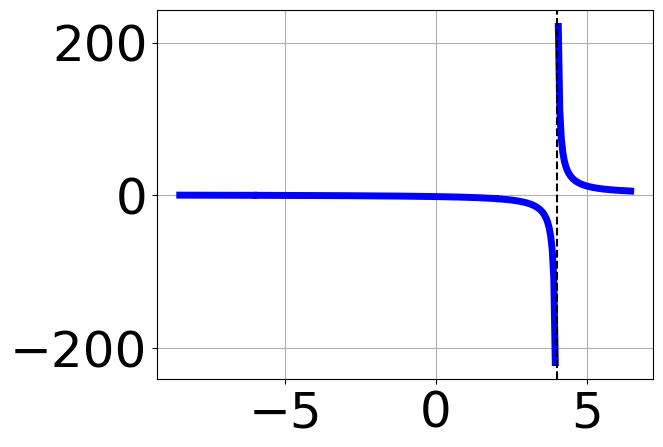
\includegraphics[width=0.5\textwidth]{../Figures/identifyGraphOfRationalFunctionA.png}
\end{center}
\begin{enumerate}[label=\Alph*.]
\item \( f(x)=\frac{x^{3} +3 x^{2} -36 x -108}{x^{3} -5 x^{2} -12 x + 36} \)
\item \( f(x)=\frac{x^{3} +3 x^{2} -36 x -108}{x^{3} -5 x^{2} -12 x + 36} \)
\item \( f(x)=\frac{x^{3} -3 x^{2} -36 x + 108}{x^{3} +5 x^{2} -12 x -36} \)
\item \( f(x)=\frac{x^{3} -1 x^{2} -44 x + 84}{x^{3} +5 x^{2} -12 x -36} \)
\item \( \text{None of the above are possible equations for the graph.} \)

\end{enumerate} }
\litem{
Determine the vertical asymptotes and holes in the rational function below.\[ f(x) = \frac{6x^{3} -25 x^{2} +29 x -10}{9x^{2} +6 x -8} \]\begin{enumerate}[label=\Alph*.]
\item \( \text{Vertical Asymptote of } x = -1.333 \text{ and hole at } x = 0.667 \)
\item \( \text{Vertical Asymptotes of } x = -1.333 \text{ and } x = 0.667 \text{ with no holes.} \)
\item \( \text{Vertical Asymptote of } x = 0.667 \text{ and hole at } x = 0.667 \)
\item \( \text{Vertical Asymptotes of } x = -1.333 \text{ and } x = 2.5 \text{ with a hole at } x = 0.667 \)
\item \( \text{Holes at } x = -1.333 \text{ and } x = 0.667 \text{ with no vertical asymptotes.} \)

\end{enumerate} }
\litem{
Determine the vertical asymptotes and holes in the rational function below.\[ f(x) = \frac{4x^{3} -8 x^{2} -11 x + 15}{6x^{2} -7 x -20} \]\begin{enumerate}[label=\Alph*.]
\item \( \text{Holes at } x = -1.333 \text{ and } x = 2.5 \text{ with no vertical asymptotes.} \)
\item \( \text{Vertical Asymptote of } x = 0.667 \text{ and hole at } x = 2.5 \)
\item \( \text{Vertical Asymptotes of } x = -1.333 \text{ and } x = 2.5 \text{ with no holes.} \)
\item \( \text{Vertical Asymptotes of } x = -1.333 \text{ and } x = -1.5 \text{ with a hole at } x = 2.5 \)
\item \( \text{Vertical Asymptote of } x = -1.333 \text{ and hole at } x = 2.5 \)

\end{enumerate} }
\litem{
Determine the horizontal and/or oblique asymptotes in the rational function below.\[ f(x) = \frac{12x^{3} +11 x^{2} -7 x -6}{3x^{3} +10 x^{2} +12 x + 4} \]\begin{enumerate}[label=\Alph*.]
\item \( \text{Vertical Asymptote of } y = -1  \)
\item \( \text{Horizontal Asymptote of } y = 4.000  \)
\item \( \text{None of the above} \)
\item \( \text{Vertical Asymptote of } y = -2.000  \)
\item \( \text{Horizontal Asymptote of } y = 0  \)

\end{enumerate} }
\end{enumerate}

\end{document}